\section{Εισαγωγή}
Τα δένδρα όπως και τα γραφήματα είναι μη γραμμικές δομές δεδομένων. Τα δένδρα επιτρέπουν ιεραρχική οργάνωση των δεδομένων όπως φαίνεται στο Σχήμα \ref{fig:binary_tree}. 

\section{Δένδρα}

Ένα δένδρο αποτελείται από κόμβους που συνδέονται μεταξύ τους με ακμές. Ο πρώτος (υψηλότερος) κόμβος του δένδρου ονομάζεται ρίζα ενώ οι κόμβοι που βρίσκονται στα άκρα του δένδρου λέγονται φύλλα. Οι κόμβοι με τους οποίους συνδέεται απευθείας ένας κόμβος ονομάζονται παιδιά του κόμβου. Αντίστοιχα, ένας κόμβος που έχει παιδιά ονομάζεται γονέας των αντίστοιχων παιδιών-κόμβων. Απόγονοι ενός κόμβου είναι οι κόμβοι για τους οποίους υπάρχει διαδρομή πραγματοποιώντας διαδοχικές μεταβάσεις από γονείς σε παιδιά. 

Τα δένδρα είναι αναδρομικές δομές από τη φύση τους. Κάθε κόμβος ενός δένδρου ορίζει έναν αριθμό από μικρότερα δένδρα, ένα για κάθε παιδί του.
 
\begin{figure}[htbp]
  \centering
  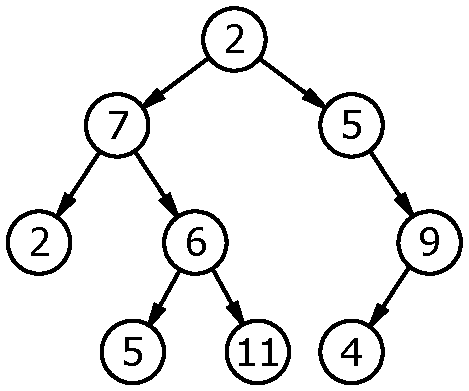
\includegraphics[width=80mm]{Binary_tree.pdf}
  \caption{Ένα απλό δένδρο \cite{wikipedia_binary_tree}}
  \label{fig:binary_tree}
\end{figure}

Ύψος δένδρου, Βάθος κορυφής

\section{Δυαδικά δένδρα}

Δυαδικό δένδρο είναι ένα δένδρο για το οποίο ισχύει ότι κάθε κόμβος έχει το πολύ δύο παιδιά \cite{parlante_binary_tree}.

\subsection{Αναζήτηση κατά βάθος}
\subsubsection{pre-order DFS}
\subsubsection{in-order DFS}
\subsubsection{post-order DFS}

\subsection{Αναζήτηση κατά πλάτος}

\lstinputlisting[caption = header file για το δυαδικό δένδρο (binary\_tree.hpp)]{lab09/binary_tree.hpp}

\lstinputlisting[caption = source file για το δυαδικό δένδρο αναζήτησης (binary\_tree.cpp)]{lab09/binary_tree.cpp}

\lstinputlisting[caption = Δοκιμή των συναρτήσεων του δυαδικού δένδρου (lab09\_ex1.cpp)]{lab09/lab09_ex1.cpp}

Η μεταγλώττιση και η εκτέλεση του κώδικα γίνεται με τις ακόλουθες εντολές:

%\lstinputlisting[style=DOS]{lab08/compile_execute2.txt}

Η δε έξοδος που παράγεται είναι η ακόλουθη:

%\lstinputlisting[style=DOS]{lab09/lab09_ex1.out}


\section{Δυαδικά δένδρα αναζήτησης}

Σε ένα δυαδικό δένδρο αναζήτησης θα πρέπει να ισχύει ότι για κάθε κόμβο Α όλες οι τιμές κλειδιών στο δένδρο αριστερά του κόμβου Α θα πρέπει να είναι μικρότερες από την τιμή κλειδιού του κόμβου Α. Αντίστοιχα, όλες οι τιμές κλειδιών στο δένδρο δεξιά του κάθε κόμβου Α θα πρέπει να είναι μεγαλύτερες από την τιμή κλειδιού του κόμβου Α.

\subsection{Υλοποίηση δυαδικού δένδρου αναζήτησης}

\lstinputlisting[caption = header file για το δυαδικό δένδρο αναζήτησης (bst.hpp)]{lab09/bst.hpp}

\lstinputlisting[caption = source file για το δυαδικό δένδρο αναζήτησης (bst.cpp)]{lab09/bst.cpp}

\lstinputlisting[caption = Δοκιμή των συναρτήσεων του δυαδικού δένδρου αναζήτησης (lab09\_ex1.cpp)]{lab09/lab09_ex2.cpp}

Η μεταγλώττιση και η εκτέλεση του κώδικα γίνεται με τις ακόλουθες εντολές:

%\lstinputlisting[style=DOS]{lab08/compile_execute2.txt}

Η δε έξοδος που παράγεται είναι η ακόλουθη:

%\lstinputlisting[style=DOS]{lab09/lab09_ex2.out}


\section{Παραδείγματα}

\subsection{Παράδειγμα 1}

Δεδομένου ενός δυαδικού δένδρου και μιας τιμής SUM ζητείται να βρεθεί το εαν υπάρχει διαδρομή από τη ρίζα του δένδρου μέχρι κάποιο κόμβο που να έχει άθροισμα κλειδιών ίσο με την τιμή SUM.

\subsection{Παράδειγμα 2}


\section{Ασκήσεις}
\begin{enumerate}
\item 
\item 
\end{enumerate}

\begin{thebibliography}{9}
\bibitem{wikipedia_binary_tree}
Wikipedia, Tree (data structure), \href{https://en.wikipedia.org/wiki/Tree_(data_structure)}{https://en.wikipedia.org/wiki/Tree\_(data\_structure)}

\bibitem{parlante_binary_tree}
Binary Trees by Nick Parlante, \href{http://cslibrary.stanford.edu/110/BinaryTrees.html}{http://cslibrary.stanford.edu/110/BinaryTrees.html}

\end{thebibliography}

